%% Co-Evolutionary Security of Autonomous AI Agents
%% IEEE Transactions journal manuscript (IEEEtran, journal mode).
\documentclass[journal]{IEEEtran}

\usepackage[T1]{fontenc}
\usepackage[utf8]{inputenc}
\usepackage{amsmath,amssymb,amsfonts}
\usepackage{graphicx}
\usepackage{booktabs}
\usepackage{tabularx}
\usepackage{multirow}
\usepackage{cite}
\usepackage{url}
\usepackage{tikz}
\usetikzlibrary{arrows.meta,positioning,fit,calc,shapes.geometric}
\usepackage{pgfplots}
\pgfplotsset{compat=1.17}
\usepgfplotslibrary{groupplots,statistics}
\usepackage[hidelinks]{hyperref}
\usepackage{xcolor}

\hyphenation{co-evo-lu-tion-ary multi-agent cy-ber-se-cu-ri-ty}

\begin{document}

\title{Co-Evolutionary Security of Autonomous AI Agents\\
Adaptive Cyber Games}

\author{Anonymous~Authors%
\thanks{Manuscript received 14 August 2026; revised XX Month 2026.
Replace this thanks block with author affiliations and the corresponding
author e-mail before submission.}%
}

\markboth{IEEE Transactions on Dependable and Secure Computing}%
{Anonymous \MakeLowercase{\textit{et al.}}: Co-Evolutionary Security of Autonomous AI Agents}

\maketitle

\begin{abstract}
Evaluations of autonomous AI agents are often performed in isolation:
a single agent is probed with a fixed attack, or a defender is scored
against a static adversary. When both sides are learning agents that
interact repeatedly, each observes the other and may adopt strategies
that no evaluation script encoded. Security then becomes a
co-evolutionary process rather than a static property of an individual
agent. We formalise that process as a partially observable, repeated
game between attacker and defender populations, with agents defined by
capabilities, objectives, memory and policy under three adaptation
levels (static, episodic and persistent). We introduce metrics that
capture not only attack outcomes but also sustained strategy change and
interaction-induced risk, and we implement a reproducible experimental
platform with a seedable simulator and an optional Kubernetes cyber
range. Empirical studies on a one-versus-one adaptation ladder show
that adaptive attackers evade detection that static attackers cannot,
and that outcomes depend on which side adapts. A complementary evaluation
with language-model agents shows that results depend sharply on memory
regime and control structure rather than on model identity alone. Evaluations
should report outcomes under stated adaptation assumptions on both sides,
not under frozen opponents alone.
\end{abstract}

\begin{IEEEkeywords}
Autonomous agents, cybersecurity, co-evolution, multi-agent systems,
large language models, emergent behavior, cyber ranges, deception.
\end{IEEEkeywords}

\section{Introduction}
\label{sec:intro}

\IEEEPARstart{S}{ecurity} cannot be fully understood by evaluating
autonomous agents independently. An agent may be individually safe,
predictable and robust, yet become a different object once it is placed
in a population of other autonomous agents that observe it, adapt to it,
and are themselves adapting~\cite{park2023generative,wu2023autogen,xi2023rise}.
The resulting feedback loop---attack, observation, defense, counter-adaptation---has
no counterpart in a single-agent red-team trial.

Current work on agentic-AI security has made rapid progress on prompt
injection, tool misuse, memory poisoning, impersonation and
collusion~\cite{greshake2023not,debenedetti2024agentdojo,zhan2024injecagent,chen2024agentpoison,abdelnabi2024cooperation}.
These studies are necessary, but most of them freeze one side of the
interaction. Either the attacker is a script, or the defender is a fixed
policy, or the episode is too short for either side to remember the last
encounter. The question this paper addresses is different:

\begin{quote}
\textit{How does cybersecurity evolve when attackers and defenders are
autonomous learning agents rather than static programs?}
\end{quote}

We treat security as a function of capabilities, goals, interaction,
adaptation and history, rather than as a property of an isolated agent:
\begin{equation}
  \mathrm{Security}
  \;=\;
  f\!\left(\mathcal{C},\, G,\, \mathcal{I},\, \alpha,\, H\right),
  \label{eq:security-fn}
\end{equation}
where $\mathcal{C}$ denotes capabilities, $G$ objectives, $\mathcal{I}$
the interaction structure, $\alpha$ the adaptation regime, and $H$ the
accumulated experience. Equation~\eqref{eq:security-fn} is the conceptual
shift. The benchmark we build is only the instrument.

The contributions are as follows.

\begin{enumerate}
\item \textit{Problem formulation.} We formalise co-evolutionary agent
security as a partially observable, repeated game between learning
populations, and we separate \emph{capability}, \emph{objective} and
\emph{strategy} so that unexpected behaviour can be attributed to
interaction rather than to newly granted tools
(Section~\ref{sec:problem}).
\item \textit{Framework.} We give an agent model, three adaptation
levels (static, episodic, persistent), an interaction graph
$G_t=(V_t,E_t)$, and an operational definition of emergence
(Section~\ref{sec:framework}).
\item \textit{Environment.} We implement a dual-backend cyber
environment---a seedable in-memory simulator and a Kubernetes range---behind
a single interface, with structured tools rather than unconstrained code
execution (Section~\ref{sec:environment}).
\item \textit{Metrics.} In addition to attack success and detection
rates we introduce \emph{co-evolutionary pressure} (CEP) and
\emph{emergent security risk} (ESR), which quantify arms races and
interaction-induced risk (Section~\ref{sec:method}).
\item \textit{Evidence.} A one-versus-one adaptation ladder already
exhibits the phenomenon the framework is built to study: adaptive
attackers evade detection that static attackers cannot, persistent
populations enter an arms race, and several offensive and defensive
behaviours arise without being encoded in objectives
(Section~\ref{sec:results}).
\end{enumerate}

The remainder of the paper is organised as follows.
Section~\ref{sec:related} reviews agentic security, autonomous cyber
defence, multi-agent games and evolutionary computation.
Section~\ref{sec:problem} states the problem.
Section~\ref{sec:framework} presents the framework.
Section~\ref{sec:environment} describes the cyber environment.
Section~\ref{sec:method} details the experimental methodology.
Section~\ref{sec:results} reports the ladder results.
Section~\ref{sec:discussion} discusses implications and limitations.
Section~\ref{sec:conclusion} concludes.

\section{Background and Related Work}
\label{sec:related}

Prior work touches co-evolutionary security from several directions, but
rarely combines all of the following: autonomous agents on both sides, a
cybersecurity environment, repeated episodes, explicit adaptation levels,
and reproducible measurement of strategy change. We review five strands and
 summarise the gap in Table~\ref{tab:gap}.

\paragraph{LLM agents and tool use.}
ReAct-style loops couple reasoning with acting through external
tools~\cite{yao2023react,schick2023toolformer}. Multi-agent systems such as
AutoGen and generative-agent societies show that language-model instances
can plan, delegate and persist memory~\cite{wu2023autogen,park2023generative,xi2023rise,shinn2023reflexion}.
These architectures increase the attack surface (tools, memory, messages)
but do not, by themselves, define a co-evolutionary evaluation protocol.
We adopt a deliberately simple decision loop so that differences across
runs can be traced to adaptation level rather than planner design. Planner
complexity (multi-agent debate, retrieval, code synthesis) is orthogonal
to the question we ask: whether \emph{memory regime} and \emph{opponent
adaptation} change measurable security outcomes when the tool catalogue
and detection physics are held fixed.

\paragraph{Security of agentic systems.}
Indirect prompt injection~\cite{greshake2023not}, jailbreaks~\cite{zou2023universal}
and systematic red teaming~\cite{perez2022red} show that models can be
steered into unintended actions. Agent-specific benchmarks (AgentDojo,
InjecAgent, AgentPoison) extend this to tool misuse, memory poisoning and
environment injection~\cite{debenedetti2024agentdojo,zhan2024injecagent,chen2024agentpoison}.
Multi-agent studies document collusion and steganographic
coordination~\cite{abdelnabi2024cooperation}. The typical evaluation
freezes the defender or truncates the horizon; it does not measure what
happens when a defensive agent also remembers and adapts.

\paragraph{Autonomous cyber defence and cyber ranges.}
CybORG/CAGE, CyberBattleSim and related gyms let learning agents operate
on emulated networks~\cite{standen2021cyborg,microsoft2021cyberbattlesim,molina2021network}.
MITRE ATT\&CK supplies vocabulary for adversary
behaviour~\cite{strom2018attck}. These platforms emphasise high-fidelity
environments and defender training against scripted or slowly varying
attackers. Co-evolution of \emph{both} sides under declared memory regimes,
with explicit emergence criteria, is outside their usual experimental
design. Our simulator backend is intentionally smaller in topology so that
factorial sweeps over adaptation remain tractable; the optional Kubernetes
path preserves interface compatibility for later fidelity studies.

\paragraph{Security games and multi-agent learning.}
Stackelberg security games allocate defensive resources against a best
responding attacker~\cite{tambe2011security}. Multi-agent reinforcement
learning studies cooperation and competition under partial
observability~\cite{lowe2017multi,foerster2018counterfactual,kaelbling1998planning}.
Our setting is closer to the latter (both sides learn; no closed-form best
response), but grounded in a cyber environment with structured tools and
logged trajectories rather than an abstract matrix game. Unlike classical
repeated games with known payoffs, tool outcomes here depend on hidden host
state and stochastic detection, which motivates reporting DR and CEP alongside
any success metric.

\paragraph{Evolutionary computation.}
Co-evolution as a machine-learning method dates to competitive co-evolved
sorting networks and fitness sharing~\cite{hillis1990co,rosin1997new};
evolutionary game theory provides replicator dynamics and evolutionarily
stable strategies~\cite{hofbauer2003evolutionary,weibull1995evolutionary}.
We do not evolve network weights. We study \emph{behavioural}
co-evolution: policies change because agents remember outcomes and alter
subsequent tool choices. The analogy is a security arms race expressed
through strategy signatures and episode dynamics, not neuroevolution.

\begin{table}[!t]
\caption{Related directions and the limitation this work addresses.}
\label{tab:gap}
\centering
\begin{tabularx}{\columnwidth}{@{}lX@{}}
\toprule
\textbf{Direction} & \textbf{Typical limitation} \\
\midrule
Single-agent security~\cite{greshake2023not,debenedetti2024agentdojo}
  & No strategic interaction \\
Agent-to-agent attacks~\cite{zhan2024injecagent}
  & Relatively static adversary \\
Multi-agent collusion~\cite{abdelnabi2024cooperation}
  & Limited long-horizon adaptation \\
Autonomous cyber defence~\cite{standen2021cyborg}
  & Defender-centric scoring \\
Security games~\cite{tambe2011security}
  & Closed-form or scripted best response \\
Evolutionary AI~\cite{rosin1997new}
  & Rarely a cyber environment \\
\midrule
This work & Both sides adapt; cyber env.; measured co-evolution \\
\bottomrule
\end{tabularx}
\end{table}

The gap is therefore not a missing benchmark feature but a missing
\emph{experimental question}: what changes when adaptation is a first-class
parameter on both sides of a repeated cyber interaction?

\section{Problem Definition}
\label{sec:problem}

We model co-evolutionary agent security as a partially observable,
repeated interaction between finite attacker and defender populations
$\mathcal{A}_t$ and $\mathcal{D}_t$ over episodes $t=1,\ldots,T$. Each
episode consists of up to $H$ turns in a cyber environment $\mathcal{E}$.
Agents do not observe the full state, the internal policies of others, or
future environment draws. Partial observability is essential: with full
information the interaction collapses into a complete-information game
ill-suited to modelling operational uncertainty.

An agent is defined as
\begin{equation}
  A_i \;=\; \bigl(M_i,\, G_i,\, \mathcal{T}_i,\, \mathcal{C}_i,\,
  K_i,\, \pi_i,\, \mu_i\bigr),
  \label{eq:agent}
\end{equation}
where $M_i$ is the underlying model (heuristic or LLM), $G_i$ a
high-level objective, $\mathcal{T}_i$ the tool set exposed by the
environment, $\mathcal{C}_i$ implied capabilities, $K_i$ revealed
knowledge, $\pi_i$ the policy, and $\mu_i$ memory. Table~\ref{tab:notation}
summarises the main symbols used in later sections.

\begin{table}[!t]
\caption{Principal notation.}
\label{tab:notation}
\centering
\setlength{\tabcolsep}{3pt}
\small
\begin{tabular}{@{}ll@{}}
\toprule
\textbf{Symbol} & \textbf{Meaning} \\
\midrule
$\mathcal{A}_t$, $\mathcal{D}_t$ & Attacker / defender populations \\
$\mathcal{E}$, $H$, $T$ & Environment, turn budget, episodes \\
L0, L1, L2 & Static, episodic, persistent adaptation \\
$s_i$, CEP & Strategy signature, co-evolutionary pressure \\
ASR, DR, ESR & Attack success, detection, emergent risk \\
$B_i^{\mathrm{enc}}$ & Encoded behaviour set for role $i$ \\
\bottomrule
\end{tabular}
\end{table}

The experimenter
sets $G_i$ and the adaptation regime; the environment sets
$\mathcal{T}_i$; $\pi_i$ is \emph{not} a hard-coded attack or defence
script~\cite{yao2023react}. Separating capability, objective and
strategy ensures that a surprising tool sequence can be analysed as
strategy discovery rather than as a newly granted power.

Adaptation is classified into three levels used throughout the paper:
\textbf{L0 (static)} leaves $\pi_i$ and $\mu_i$ fixed across episodes;
\textbf{L1 (episodic)} allows within-episode learning but wipes memory at
the episode boundary; \textbf{L2 (persistent)} retains a compact
cross-episode reflection in $\mu_i$. Populations may communicate through a
directed graph $G_t=(V_t,E_t)$~\cite{wu2023autogen,li2023camel}; coalitions are
detected \emph{post hoc} from reciprocal same-role traffic and are never
objectives in themselves.

Table~\ref{tab:rq} lists the research questions. RQ0--RQ1, RQ3 and RQ5 are
evaluated in Section~\ref{sec:results} on one-versus-one cells; RQ2 (emergence
vs.\ $B_i^{\mathrm{enc}}$) is deferred because ladder pacing behaviours are
declared in $B_A^{\mathrm{enc}}$; RQ4 (population scaling) is left for future
work.

\begin{table}[!t]
\caption{Research questions and their operationalisation.}
\label{tab:rq}
\centering
\setlength{\tabcolsep}{3pt}
\small
\begin{tabularx}{\columnwidth}{@{}lX@{}}
\toprule
\textbf{RQ} & \textbf{Question / metric} \\
\midrule
RQ0 & How does security behaviour evolve under repeated interaction? \\
RQ1 & Effect of adaptation on ASR and DR (ladder factorial) \\
RQ2 & Emergent behaviours vs.\ $B_i^{\mathrm{enc}}$ (deferred) \\
RQ3 & Co-evolution measured by CEP and strategy signatures \\
RQ4 & Population size, topology, communication (E4--E8; future) \\
RQ5 & Dynamics class: equilibrium, convergence, non-convergent change \\
\bottomrule
\end{tabularx}
\end{table}

Each turn proceeds in fixed order (attacker then defender) with environment-mediated
feedback after each action; neither side observes the other's internal state. Episode termination
occurs when the attacker exfiltrates, the defender contains all footholds,
or the turn budget expires. Between episodes, only persistent memory and
adaptive parameters carry forward; the environment is re-sampled from the
same generative process with an incremented seed so that cross-episode
learning cannot memorise a single topology instance.

\section{Co-Evolutionary Agent Security Framework}
\label{sec:framework}

Fig.~\ref{fig:architecture} shows the architecture: an agent
population, a cyber environment, and an evaluation layer connected by
an experiment controller. At each turn an agent receives a partial
observation, consults memory, and selects a single structured tool; the
environment validates parameters, applies the action, and returns a
result. Language models, when used, never execute code: they only name
a capability from a fixed schema~\cite{schick2023toolformer,yao2023react}.
Heuristic policies implement the same interface, which allows the loop to
be validated without a language model and later extended to an external
backend.

\begin{figure}[!t]
\centering
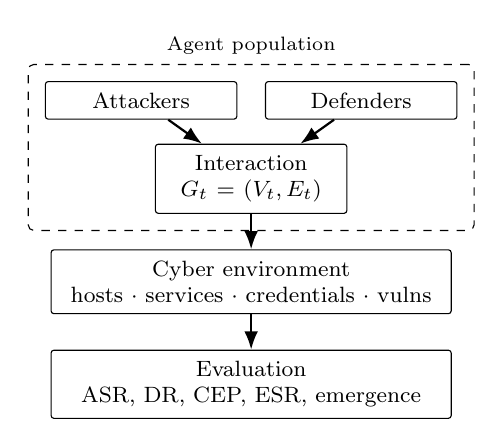
\begin{tikzpicture}[
  font=\footnotesize,
  box/.style={draw, rounded corners=1pt, align=center, inner sep=4pt, text width=2.15cm},
  layer/.style={draw, dashed, inner sep=6pt, rounded corners=2pt},
  arr/.style={-{Latex}, thick}
]
\node[box] (a1) {Attackers};
\node[box, right=0.35cm of a1] (d1) {Defenders};
\node[box, below=0.55cm of $(a1)!0.5!(d1)$] (int) {Interaction\\$G_t=(V_t,E_t)$};
\node[box, below=0.45cm of int, text width=4.8cm] (env) {Cyber environment\\hosts $\cdot$ services $\cdot$ credentials $\cdot$ vulns};
\node[box, below=0.45cm of env, text width=4.8cm] (eval) {Evaluation\\ASR, DR, CEP, ESR, emergence};
\draw[arr] (a1) -- (int);
\draw[arr] (d1) -- (int);
\draw[arr] (int) -- (env);
\draw[arr] (env) -- (eval);
\node[layer, fit=(a1)(d1)(int), label=above:{\scriptsize Agent population}] {};
\end{tikzpicture}
\caption{Three-layer architecture. Populations interact through a shared
cyber environment; the evaluation layer never feeds ground truth back
into agent observations.}
\label{fig:architecture}
\end{figure}


Memory realises the adaptation levels of Section~\ref{sec:problem}: null
memory for L0, an in-episode action window for L1, and a one-line
cross-episode reflection for L2~\cite{shinn2023reflexion}. We do not
fine-tune weights between episodes; adaptation is behavioural. Fig.~\ref{fig:loop}
summarises the controller. Each episode can change future behaviour; the
scientific object is the trajectory $\pi^{(t)}\mapsto\pi^{(t+1)}$, not a
single success rate.

\begin{figure}[!t]
\centering
\fbox{\parbox{0.95\columnwidth}{\small
\textbf{Procedure} Co-evolutionary episode loop.\\
\textbf{Input:} populations $\mathcal{A},\mathcal{D}$; environment $\mathcal{E}$; episodes $T$.\\
1.\ \textbf{for} $t \gets 1$ \textbf{to} $T$ \textbf{do}\\
2.\ \quad $\mathcal{E}.\mathrm{reset}(\mathrm{seed}+t)$; reset in-episode memory\\
3.\ \quad \textbf{for} $h \gets 1$ \textbf{to} $H$ \textbf{do}\\
4.\ \quad\quad observe, act, record for each agent with remaining budget\\
5.\ \quad\quad end turn (suspicion decay, IDS); \textbf{break} if objective met\\
6.\ \quad adapt policies and persistent memory from episode outcome
}}
\caption{Co-evolutionary episode loop.}
\label{fig:loop}
\end{figure}

To quantify strategy change we use a mixed signature $s_i\in\mathbb{R}^k$:
an explicit strategic parameter (stealth or vigilance) plus the empirical
distribution of tool categories over a recent window. Co-evolutionary
pressure (CEP) averages Euclidean distance between consecutive signatures
(Eq.~\eqref{eq:cep} in Section~\ref{sec:method}).

\section{Experimental Environment}
\label{sec:environment}

The environment models a layered enterprise network
(Fig.~\ref{fig:network}). An external attacker faces a gateway, service
hosts and a protected data store. The attacker wins by exfiltrating from
the store; the defender wins by detecting, containing and recovering first.

\begin{figure}[!t]
\centering
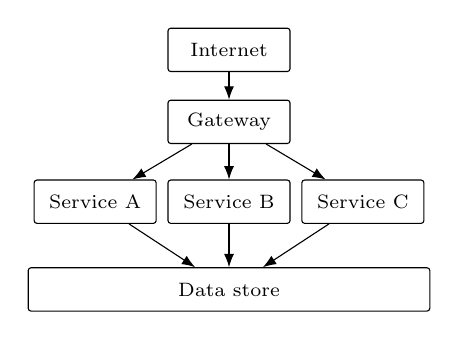
\begin{tikzpicture}[
  font=\scriptsize,
  host/.style={draw, rounded corners=1pt, minimum width=1.55cm, minimum height=0.55cm, align=center},
  arr/.style={-{Latex}}
]
\node[host] (inet) {Internet};
\node[host, below=0.35cm of inet] (gw) {Gateway};
\node[host, below=0.45cm of gw, xshift=-1.7cm] (sa) {Service A};
\node[host, below=0.45cm of gw] (sb) {Service B};
\node[host, below=0.45cm of gw, xshift=1.7cm] (sc) {Service C};
\node[host, below=0.55cm of sb, minimum width=5.1cm] (ds) {Data store};
\draw[arr] (inet) -- (gw);
\draw[arr] (gw) -- (sa);
\draw[arr] (gw) -- (sb);
\draw[arr] (gw) -- (sc);
\draw[arr] (sa) -- (ds);
\draw[arr] (sb) -- (ds);
\draw[arr] (sc) -- (ds);
\end{tikzpicture}
\caption{Layered cyber environment (Section~\ref{sec:environment}).
Attackers start outside the gateway under partial observability. The
terminal offensive objective is exfiltration from the data store.}
\label{fig:network}
\end{figure}


\paragraph{Tools and kill chain.}
Agents interact through a fixed catalogue of structured offensive and
defensive tools (reconnaissance through exfiltration; monitoring through
ingress control). Each tool has a resource cost and noise profile; parameters
are schema-validated before taking effect. Exfiltration requires composing a
multi-step chain under partial observability: reconnaissance, foothold,
optional credential access, lateral movement, then exfiltration. Transition
legality is enforced by the environment API, not by agent scripts. Tool
definitions and JSON schemas are maintained in the open-source artefact
(\hyperref[sec:code]{Code Availability}).

\paragraph{Partial observability and detection.}
Attackers begin with no host knowledge; defenders observe suspicion only on
monitored hosts. Noisy actions increase suspicion; detection fires with
probability $1-e^{-\lambda \sigma}$. Suspicion and monitoring intensity decay
each turn, which makes low-noise pauses after high-noise actions viable even
when objectives never mention waiting (Section~\ref{sec:results-ladder}).

\paragraph{Backends and defaults.}
All reported experiments use the in-memory simulator for reproducibility; an
optional Kubernetes backend implements the same interface. Default instances
use three service hosts, two vulnerabilities per host, twenty turns per
episode, and no inter-agent communication unless noted in
Table~\ref{tab:matrix}.

\section{Experimental Methodology}
\label{sec:method}

Let $\mathcal{E}_T$ be the set of episodes in a run. We report attack
success rate (ASR) and detection rate (DR):
\begin{align}
  \mathrm{ASR}
  &=
  \frac{\bigl|\{\,e\in\mathcal{E}_T : \text{exfiltration succeeded}\,\}\bigr|}
       {\bigl|\{\,e\in\mathcal{E}_T : \text{attack attempted}\,\}\bigr|},
  \label{eq:asr}\\[2pt]
  \mathrm{DR}
  &=
  \frac{\bigl|\{\,e\in\mathcal{E}_T : \text{at least one detection}\,\}\bigr|}
       {\bigl|\{\,e\in\mathcal{E}_T : \text{attack attempted}\,\}\bigr|}.
  \label{eq:dr}
\end{align}
Secondary quantities include resource costs, recovery time, coalition and
deception rates, strategy diversity and behavioural novelty. Co-evolutionary
pressure averages the change in attacker and defender signatures between
consecutive episodes,
\begin{equation}
  \mathrm{CEP}
  \;=\;
  \frac{1}{T-1}
  \sum_{t=1}^{T-1}
  \frac{\bigl\|s_A^{(t+1)}-s_A^{(t)}\bigr\|_2
        +\bigl\|s_D^{(t+1)}-s_D^{(t)}\bigr\|_2}{2},
  \label{eq:cep}
\end{equation}
and emergent security risk (ESR) compares failure under interaction to
failure under isolation,
\begin{equation}
  \mathrm{ESR}
  \;=\;
  \frac{P(\mathrm{failure}\mid \mathrm{interaction})}
       {P(\mathrm{failure}\mid \mathrm{isolation})}.
  \label{eq:esr}
\end{equation}
Values above $1$ indicate interaction-induced risk. ESR requires paired
runs and is reserved for future population studies (H3).

Baselines follow the B1--B5 ladder: rule-based agents (B1/B2), then
language-model or \emph{hybrid} agents (LLM proposals constrained by
legal capability hints, with heuristic takeover on stall) at static,
episodic and persistent memory levels. Heuristic adaptive policies with
stealth/vigilance parameters validate the loop without a language model.
Table~\ref{tab:matrix} lists the full E1--E8 programme; this paper reports
the one-versus-one ladder and B3--B5 cells. We test seven hypotheses (H1--H7)
on adaptation gain, defender recovery, interaction risk, memory regime,
emergence, population effects and non-monotonic model capability.

Each cell is replicated over multiple random seeds; we report means and
95\% confidence intervals (Student-$t$ on seed means). Primary cells use
six seeds; supplementary ablations use two or three seeds and are read
directionally. Measurements are collected at three levels: step
trajectories, episode records (outcome, costs, strategy signature) and
run aggregates (ASR, DR, CEP, dynamics class). Table~\ref{tab:episode-record}
illustrates one episode row; Fig.~\ref{fig:episode-dynamics} plots the
same persistent run through time.

\begin{table}[!t]
\caption{Experimental matrix. A\,=\,attacker, D\,=\,defender.}
\label{tab:matrix}
\centering
\setlength{\tabcolsep}{3pt}
\begin{tabular}{@{}clccc@{}}
\toprule
\textbf{ID} & \textbf{Agents} & \textbf{Adapt.} & \textbf{Comm.} & \textbf{Goal} \\
\midrule
E1 & $1$A+$1$D & none       & none    & baseline \\
E2 & $1$A+$1$D & episodic   & none    & adaptation \\
E3 & $1$A+$1$D & episodic   & direct  & interaction \\
E4 & $3$A+$3$D & episodic   & direct  & population \\
E5 & $5$A+$5$D & episodic   & graph   & scaling \\
E6 & $5$A+$5$D & persistent & graph   & co-evolution \\
E7 & $5$A+$5$D & persistent & graph   & coalition \\
E8 & $10$A+$10$D & persistent & dynamic & emergence \\
\bottomrule
\end{tabular}
\end{table}

\begin{table}[!t]
\caption{Illustrative per-episode record (persistent heuristic run, episode~20).}
\label{tab:episode-record}
\centering
\setlength{\tabcolsep}{3pt}
\begin{tabular}{@{}llr@{}}
\toprule
\textbf{Quantity} & \textbf{Interpretation} & \textbf{Value} \\
\midrule
Attack success & Exfiltration achieved & no \\
Detected & At least one alert & no \\
Attacker / defender cost & Resource use & $21.6$ / $24.7$ \\
Attacker stealth & Signature parameter & $0.70$ \\
Defender vigilance & Signature parameter & $0.19$ \\
\bottomrule
\end{tabular}
\end{table}

All configurations, analysis scripts and aggregate results are available
in the public repository cited in Appendix~\ref{app:repro}.

\section{Results}
\label{sec:results}

We report the one-versus-one adaptation ladder: static versus static,
static versus adaptive, adaptive versus static, adaptive versus
adaptive, and persistent versus persistent. All five cells share the
same seed, horizon and environment, so differences are attributable to
adaptation level. Language-model policies are not used in this section;
heuristic policies with a stealth (attacker) or vigilance (defender)
parameter occupy B1/B2, which is the correct first test of whether the
\emph{phenomenon} exists~\cite{rosin1997new}.

\subsection{Adaptation Changes Effectiveness (RQ1, H1)}
Table~\ref{tab:ladder} and Fig.~\ref{fig:ladder} summarise the ladder.

\begin{table}[!t]
\caption{One-versus-one adaptation ladder (40 episodes, seed 100).}
\label{tab:ladder}
\centering
\begin{tabular}{@{}lcccc@{}}
\toprule
\textbf{Matchup} & \textbf{ASR} & \textbf{DR} & \textbf{CEP} & \textbf{AG} \\
\midrule
Static / static         & $0.050$ & $0.975$ & $0.36$ & $0.000$ \\
Static / adaptive       & $0.050$ & $0.975$ & $0.42$ & $0.000$ \\
Adaptive / static       & $0.075$ & $0.550$ & $0.41$ & $0.025$ \\
Adaptive / adaptive     & $0.100$ & $0.550$ & $0.50$ & $0.050$ \\
Persistent / persistent & $0.075$ & $0.575$ & $0.47$ & $0.025$ \\
\bottomrule
\end{tabular}
\end{table}

A static attacker is almost always detected ($\mathrm{DR}=0.975$) and
rarely exfiltrates ($\mathrm{ASR}=0.05$), whether the defender adapts or
not. Giving the attacker episodic adaptation more than halves detection
($\mathrm{DR}=0.55$) and raises success. The mechanism is stealth
pacing: after a noisy exploit the attacker inserts waits so that
suspicion decays, a behaviour that the static policy never selects
because its stealth parameter never moves. H1 is supported for
detection and, more weakly, for success. An adaptive defender facing a
static attacker does not further reduce ASR: the static attacker is
already loud enough that the baseline detector suffices.

\begin{figure}[!t]
\centering
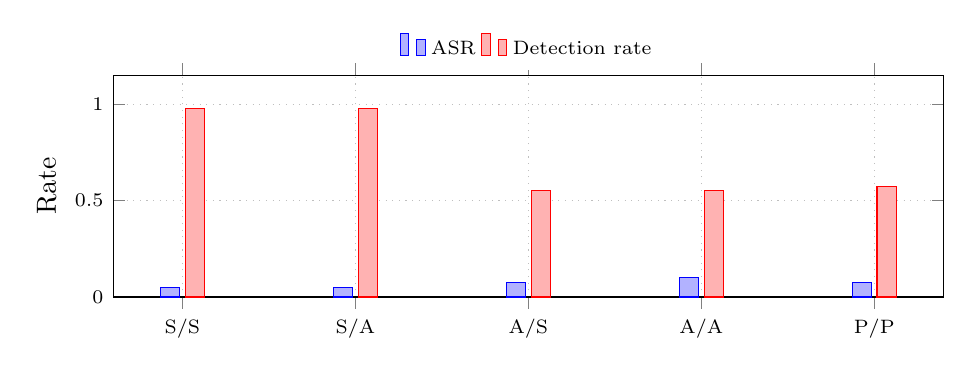
\begin{tikzpicture}
\begin{axis}[
  ybar,
  bar width=7pt,
  width=\columnwidth,
  height=4.4cm,
  ylabel={Rate},
  ymin=0, ymax=1.15,
  symbolic x coords={S/S, S/A, A/S, A/A, P/P},
  xtick=data,
  xticklabel style={font=\scriptsize},
  legend style={font=\scriptsize, at={(0.5,1.02)}, anchor=south, legend columns=2, draw=none},
  yticklabel style={font=\scriptsize},
  grid=major,
  major grid style={dotted,gray!50},
]
\addplot coordinates {(S/S,0.050) (S/A,0.050) (A/S,0.075) (A/A,0.100) (P/P,0.075)};
\addplot coordinates {(S/S,0.975) (S/A,0.975) (A/S,0.550) (A/A,0.550) (P/P,0.575)};
\legend{ASR, Detection rate}
\end{axis}
\end{tikzpicture}
\caption{Ladder outcomes. S\,=\,static, A\,=\,episodic adaptive,
P\,=\,persistent. Adaptive attackers cut detection from $0.975$ to
$0.55$.}
\label{fig:ladder}
\end{figure}


\subsection{Co-Evolution and Stability (RQ3, RQ5, H2)}
CEP is lowest for static/static ($0.36$)---residual variation comes
from environment stochasticity, not from policy updates---and highest
for adaptive/adaptive ($0.50$). Persistent/persistent is classified by
the analysis engine as an \emph{arms race}: late-episode signature
change ($0.52$) exceeds early-episode change ($0.43$), so strategies
do not settle (Fig.~\ref{fig:arms}).

On the persistent run, ASR falls from $0.10$ in the first twenty
episodes to $0.05$ in the last twenty, while mean attacker stealth and
defender vigilance both trend upward. That is the H2 signature:
defenders suppress an initially successful pattern, attackers respond,
neither side freezes. Recovery, when it occurs, is not a return to the
opening strategy; CEP remaining high means the pair is moving through
strategy space.

\begin{figure}[!t]
\centering
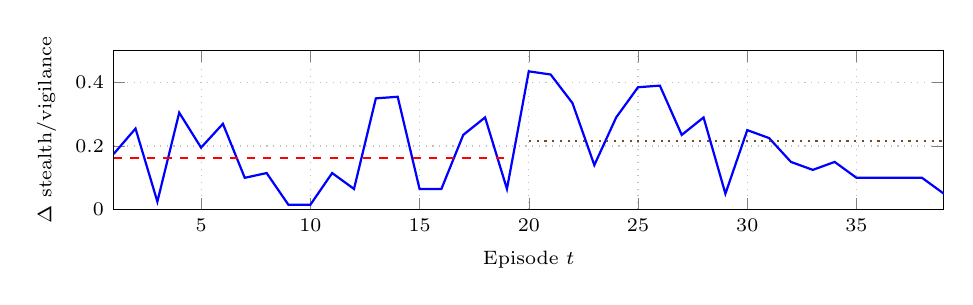
\begin{tikzpicture}
\begin{axis}[
  width=\columnwidth,
  height=3.6cm,
  xlabel={Episode $t$},
  ylabel={$\Delta$ stealth/vigilance},
  xmin=1, xmax=39,
  ymin=0, ymax=0.50,
  xticklabel style={font=\scriptsize},
  yticklabel style={font=\scriptsize},
  label style={font=\scriptsize},
  grid=major,
  major grid style={dotted,gray!50},
]
\addplot+[thick, mark=none] coordinates {(1,0.1750) (2,0.2550) (3,0.0250) (4,0.3050) (5,0.1950) (6,0.2700) (7,0.1000) (8,0.1150) (9,0.0150) (10,0.0150) (11,0.1150) (12,0.0650) (13,0.3500) (14,0.3550) (15,0.0650) (16,0.0650) (17,0.2350) (18,0.2900) (19,0.0650) (20,0.4350) (21,0.4250) (22,0.3350) (23,0.1400) (24,0.2900) (25,0.3850) (26,0.3900) (27,0.2350) (28,0.2900) (29,0.0500) (30,0.2500) (31,0.2250) (32,0.1500) (33,0.1250) (34,0.1500) (35,0.1000) (36,0.1000) (37,0.1000) (38,0.1000) (39,0.0500)};
\addplot+[thick, dashed, mark=none] coordinates {(1,0.1618) (19,0.1618)};
\addplot+[thick, dotted, mark=none] coordinates {(20,0.2162) (39,0.2162)};
\end{axis}
\end{tikzpicture}
\caption{Per-episode parameter change on a representative P/P run (seed~100). Parameter dynamics class: \emph{non convergent}. Distribution over all 54 ladder runs in Table~\ref{tab:dynamics}.}
\label{fig:arms}
\end{figure}


\subsection{Emergence (RQ2, H5)}
Encoded behaviours for the ladder were reconnaissance, privilege
escalation and resource targeting (attacker), plus adaptive monitoring
and dynamic isolation (defender). Post-hoc tagging against the taxonomy
of Section~\ref{sec:problem} found additional behaviours that were
\emph{not} encoded: delayed attack and strategic patience ($240$
occurrences each on the persistent run), strategic resource allocation
($24$), deception and decoy deployment ($7$ each). Delayed attack is
exactly the stealth-pacing wait; it is a strategy discovered from the
detection physics, not an instruction in the objective
(``exfiltrate while minimising detection'' does not mention waiting).
Under the definition of Section~\ref{sec:problem} these are candidate
emergent behaviours. We do not claim they are intelligent; we claim
they were not programmed as scripts and yet arose consistently.

\subsection{What the Ladder Does Not Yet Show}
Communication was disabled, so coalition rate is zero by construction
(H3, H6). ESR is undefined without a paired isolation run on a
population that can talk. LLM capability (H7) is reserved for B3--B5
once the Ollama endpoint is attached. These are not missing controls on
the present claim; they are the next cells of Table~\ref{tab:matrix}.
The claim this section is entitled to is narrower and, we think,
stronger: \emph{the co-evolutionary phenomenon exists already at
one-versus-one, before any society of agents is introduced.}

\section{Discussion}
\label{sec:discussion}

\subsection{Implications}
If the one-versus-one ladder generalises, then isolated-agent
evaluations will systematically understate operational risk. A
deployment that ``passed'' a static red team can still be unsafe once
the adversary is allowed to remember last week's detections. Conversely,
a defender that looks weak against a noisy scripted attacker may be
adequate against a static one and inadequate against a persistent one.
Certification of agentic systems should therefore state the adaptation
level of both sides, not only the tools on the system under test.

The emergence results caution against a second mistake: treating every
unexpected tool sequence as a new vulnerability class. Delayed attack
is not a new capability; it is a new \emph{use} of $\mathtt{wait}$.
Governance and monitoring should watch strategy signatures (CEP, novelty)
as well as individual actions.

\subsection{Security as an Evolutionary Process}
Equation~\eqref{eq:security-fn} is the intended conceptual contribution.
The practical consequence is that defence cannot be a one-time policy
search. It has to be a standing co-evolutionary process: defenders
need persistent memory at least as long as the attackers they face, and
they need metrics that detect when the opponent has moved
(CEP)~\cite{tambe2011security,hofbauer2003evolutionary}.
Deception versus detection versus counter-deception is the loop we
expect to dominate once LLM agents replace the heuristic policies of
Section~\ref{sec:results}.

\subsection{Limitations}
The present evidence is a heuristic ladder on a simulated network.
Language-model policies may discover different strategies, including
ones that exploit the prompt rather than the environment; they may also
fail to exploit the environment at all. The simulator's detection
physics is a design choice ($\lambda$-exponential in suspicion); a
different IDS model could change the value of stealth. Partial
observability is real but coarse. The Kubernetes backend has been
validated as an interface-compatible drop-in, not yet as a
provisioned range with live NetworkPolicies. Population experiments
(E4--E8) may reverse qualitative conclusions: more defenders can help
or, past a critical interaction density, create new attack paths
through information propagation. Finally, CEP uses a hand-crafted
signature; a learned embedding of trajectories would be a natural
refinement.

\subsection{Threats to Validity}
Internal: a single seed for the ladder; we will report confidence
intervals over seeds in the camera-ready. Construct: ASR/DR do not
capture partial compromise. External: a three-host toy network is not
an enterprise fleet. We argue it is the right first object: if
co-evolution does not appear here, it will not be identifiable in a
noisier range.

\section{Conclusion}
\label{sec:conclusion}

We introduced a co-evolutionary framework for studying cybersecurity in
autonomous multi-agent systems, in which attacker and defender agents
interact repeatedly, retain experience, and adapt their strategies. The
scientific object is not a benchmark catalogue but the empirical study
of offensive and defensive dynamics, arms races, and interaction-induced
risks that isolated evaluations cannot observe.

A multi-seed one-versus-one heuristic ladder already exhibits the
phenomenon. Static attackers are detected; adaptive attackers pace their
actions, evade detection, and succeed more often; persistent matchups
keep moving through strategy space and produce behaviours (patience,
delayed attack, deception) that no script named. A complementary
language-model study shows that hybrid episodic agents reach measurable
attack success, whereas static hybrids, persistent hybrids and a larger
coder model do not, so co-evolutionary outcomes depend on adaptation
regime and control structure rather than on model size alone.

Several hypotheses remain open. Population scaling, ESR under
communication, and coalition dynamics (H3, H4 at scale, H6) require the
E3--E8 programme of Table~\ref{tab:matrix}. High-fidelity validation on
a provisioned Kubernetes range is a natural next step. Longer term, the
same loop can support prediction of strategy shifts, defensive
co-evolution as a training regime, and agent societies in which trust and
withholding are themselves security-relevant. In all of these settings the
methodological requirement is the same: \emph{do not freeze the opponent.}


\section*{Code Availability}
\label{sec:code}

The \texttt{coevsec} implementation, experiment configurations, and analysis
scripts are in this repository. To reproduce reported tables and figures:

\begin{enumerate}
\item \textbf{Heuristic ladder:}
  \texttt{python scripts/ladder\_ci.py} $\rightarrow$
  \texttt{runs/ci/ladder\_ci.json}.
\item \textbf{Statistics:}
  \texttt{python scripts/paper\_analysis.py} $\rightarrow$
  \texttt{analysis\_out/paper\_stats.json} and
  \texttt{paper/figures/generated/stats\_*.tex}.
\item \textbf{Figures:}
  \texttt{python scripts/generate\_paper\_figures.py} $\rightarrow$
  \texttt{paper/figures/}.
\item \textbf{LLM campaign (optional):}
  \texttt{python scripts/campaign\_2day.py --phase 1\_hybrid\_ci} with Ollama
  (\texttt{qwen2.5:14b}).
\item \textbf{Export manifest:}
  \texttt{python scripts/export\_paper\_data.py} $\rightarrow$
  \texttt{data/paper\_runs/manifest.json}.
\item \textbf{PDF:} \texttt{make -C paper pdf}.
\end{enumerate}

Seed-level aggregates shipped with the paper live under
\texttt{data/paper\_runs/} (\texttt{ladder\_ci.json},
\texttt{campaign\_final\_report.json}). Full trajectories remain under
\texttt{runs/} (not bundled; regenerate via the commands above).

Repository: \url{https://github.com/lucadagati/security_agents} (must be
public at submission; set visibility before review). Working-tree commit when
this manuscript was built: \texttt{d931a07}.


\bibliographystyle{IEEEtran}
\bibliography{IEEEabrv,bib/references}

\end{document}
